\documentclass{article}

% Language setting
% Replace `english' with e.g. `spanish' to change the document language
\usepackage[english]{babel}

% Set page size and margins
% Replace `letterpaper' with `a4paper' for UK/EU standard size
\usepackage[letterpaper,top=2cm,bottom=2cm,left=3cm,right=3cm,marginparwidth=1.75cm]{geometry}

% Useful packages
\usepackage{enumerate}
\usepackage[shortlabels]{enumitem}
\usepackage{amsmath, amsfonts, amssymb, mathtools}
\usepackage{graphicx}
\usepackage[colorlinks=true, allcolors=blue]{hyperref}
\usepackage[table]{xcolor}  % For coloring rows
\usepackage{ tipa }
\usepackage[section]{placeins}

% For drawing state machine
\usepackage{tikz}
\usetikzlibrary{automata} % Import library for drawing automata
\usetikzlibrary{positioning} % ...positioning nodes
\usetikzlibrary{arrows} % ...customizing arrows
\tikzset{
    node distance=3cm, % Minimum distance between two nodes. Change if necessary.
    every state/.style={ % Sets the properties for each state
        thick,
        fill=gray!10
    },
    initial text={}, % No label on start arrow
    double distance=2pt, % Adjust appearance of accept states
    bend angle=15,
    every edge/.style={ % Sets the properties for each transition
        draw,
        ->,>=stealth, % Makes edges directed with bold arrowheads
        auto,
        thick
    }
}
            
\let\epsilon\varepsilon

\newcommand{\N}{\mathbb{N}}

\title{
Cyber Physical Systems - Discrete Models \\
[0.2em]Exercise Sheet 3 Solution
}
\author{
  Alper Ari\\
  \texttt{aa508@uni-freiburg.edu}
  \and
  Onur Sahin\\
  \texttt{os141@uni-freiburg.de}
}
\date{\today}

\begin{document}
\maketitle

\section*{Exercise 1: Intersection of $\omega$-regular languages}
\begin{enumerate}[(a)]
     \item{
        $L_1$: It is certain that \textit{a} is not infinite. However, \textit{b} or \textit{c} can be infinite.\\
        $L_2$: It is certain that \textit{b} is infinite. However, \textit{a} and \textit{c} can also be infinite.\\
        $L_1 \bigcap L_2$: It is certain that \textit{a} is not infinite and \textit{b} is infinite. However, \textit{c} can be infinite.
     }
     \begin{figure}[ht] % ’ht’ tells LaTeX to place the figure ’here’ or at the top of the page
        \centering % centers the figure
        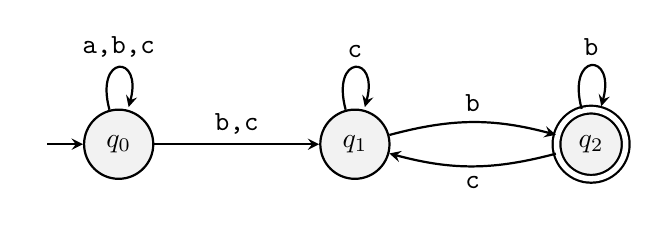
\begin{tikzpicture}
            \node[state, initial] (q0) {$q_0$};
            \node[state, right of=q0] (q1) {$q_1$};
            \node[state, accepting, right of=q1] (q2) {$q_2$};
            
            \draw (q0) edge[loop above] node {\tt a,b,c} (q0);
            \draw (q0) edge node {\tt b,c} (q1);
            \draw (q1) edge[loop above] node {\tt c} (q1);

            \draw (q1) edge[bend left] node {\tt b} (q2);
            \draw (q2) edge[bend left] node {\tt c} (q1);

            \draw (q2) edge[loop above] node {\tt b} (q2);
        \end{tikzpicture}
        \caption{Büchi automaton A that accepts intersection of $L_1$ and $L_2$ }
        \label{fig:state-machine-l1}
    \end{figure}

    \item{
        $L_1$: It is certain that \textit{a} is infinite. However, \textit{b} can also be infinite.\\
        $L_2$: It is certain that \textit{b} is infinite. However, \textit{a} can also be infinite.\\
        $L_1 \bigcap L_2$: It is certain that \textit{a} and \textit{b} infinite.
    }
     \begin{figure}[ht] % ’ht’ tells LaTeX to place the figure ’here’ or at the top of the page
        \centering % centers the figure
        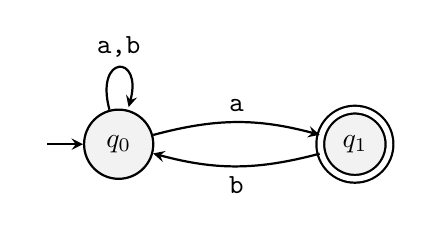
\begin{tikzpicture}
            \node[state, initial] (q0) {$q_0$};
            \node[state, accepting, right of=q0] (q1) {$q_1$};
            
            \draw (q0) edge[loop above] node {\tt a,b} (q0);
            \draw (q0) edge[bend left] node {\tt a} (q1);
            \draw (q1) edge[bend left] node {\tt b} (q0);
        \end{tikzpicture}
        \caption{Büchi automaton A that accepts intersection of $L_1$ and $L_2$ }
        \label{fig:state-machine-l1}
    \end{figure}


    \item{
        $L_1$: It is certain that \textit{a} is not infinite. However, \textit{b} can be infinite.\\
        $L_2$: It is certain that if there is \textit{b} at any position, regardless of finite or infinite words, there must be \textit{a} right next to it. However, \textit{a} can be infinite. Yet, \textit{b} can also be infinite as long as it follows \textit{a}, which means both are infinite only if they are together.\\
        $L_1 \bigcap L_2$: $\emptyset$ (It is certain that \textit{a} is not infinite. And \textit{b} cannot be infinite since \textit{a} is not infinite) \\
        Since there is no infinite run containing an accepting state on the Büchi Automaton, the intersection is an empty language.
    }
    \begin{figure}[ht] % ’ht’ tells LaTeX to place the figure ’here’ or at the top of the page
        \centering % centers the figure
        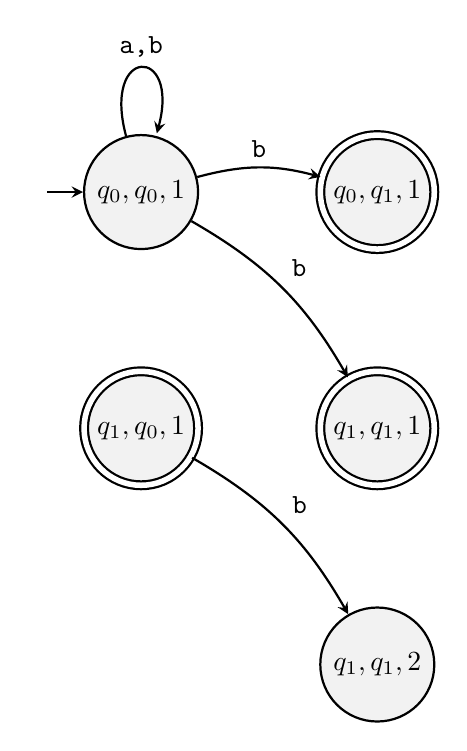
\begin{tikzpicture}
            \node[state, initial] (q0q0_1) {$q_0, q_0, 1$};
            \node[state, accepting, right of=q0q0_1] (q0q1_1) {$q_0, q_1, 1$};
            \node[state, accepting, below of=q0q1_1] (q1q1_1) {$q_1, q_1, 1$};
            \node[state, accepting, below of=q0q0_1] (q1q0_1) {$q_1, q_0, 1$};
            \node[state, below of=q1q1_1] (q1q1_2) {$q_1, q_1, 2$};
            
            \draw (q0q0_1) edge[loop above] node {\tt a,b} (q0q0_1);
            \draw (q0q0_1) edge[bend left] node {\tt b} (q0q1_1);
            \draw (q0q0_1) edge[bend left] node {\tt b} (q1q1_1);
            \draw (q1q0_1) edge[bend left] node {\tt b} (q1q1_2);
        \end{tikzpicture}
        \caption{Büchi automaton A that accepts intersection of $L_1$ and $L_2$ }
        \label{fig:state-machine-l1}
    \end{figure}
    
\end{enumerate}

\newpage

\section*{Exercise 2: Transition Systems}
\begin{enumerate}[(a)]
    \item{The model represents a case or lock which can be opened by inserting a ticket. Red light appears if locked. Otherwise, green light appears.}
    \begin{figure}[!htb]
        \centering
        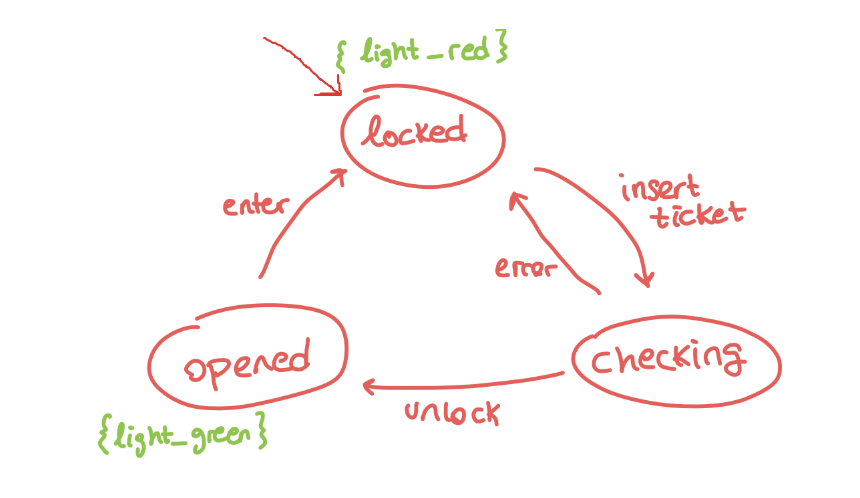
\includegraphics[width=3in]{images/2a.png}
        \caption{Transition System}
        \label{fig:2a}
    \end{figure}

    \item{Mathematical definition of given transition system is as follows:}
        \begin{equation*}
        \centering
            \begin{split}
                S &= \{1,2,3,4\} \\
                Act &= \{\text{close\textunderscore door}, \text{open\textunderscore door}, \text{go\textunderscore up}, \text{go\textunderscore down}\}\\
                S_0 &= \{4, 1\}\\
                L(4) &= \{\text{open, top\textunderscore floor}\}\\
                L(3) &= \{\text{top\textunderscore floor}\}\\
                L(2) &= \{\text{ground\textunderscore floor}\}\\
                L(1) &= \{\text{open, ground\textunderscore floor}\}\\
                % \text{The door is closed in states 2 and 3.}
            \end{split}
        \end{equation*}
        Transitions are as follows:\\
        \begin{multline*}
        \longrightarrow = \{
        (4, \text{close\textunderscore door}, 3), (3, \text{open\textunderscore door}, 4), (3, \text{go\textunderscore down}, 2),\\
        (2, \text{go\textunderscore up}, 3), (2, \text{open\textunderscore door}, 1), (1, \text{close\textunderscore door}, 2)\} 
        \end{multline*}    
        \\
        And the door is open at states 2 and 3.
\end{enumerate}

\newpage

\section*{Exercise 3: Crossroads Traffic Lights}

\begin{enumerate}[(a)]
    \item{The traffic lights do not synchronize with each other.}
    \begin{figure}[!htb]
        \centering
        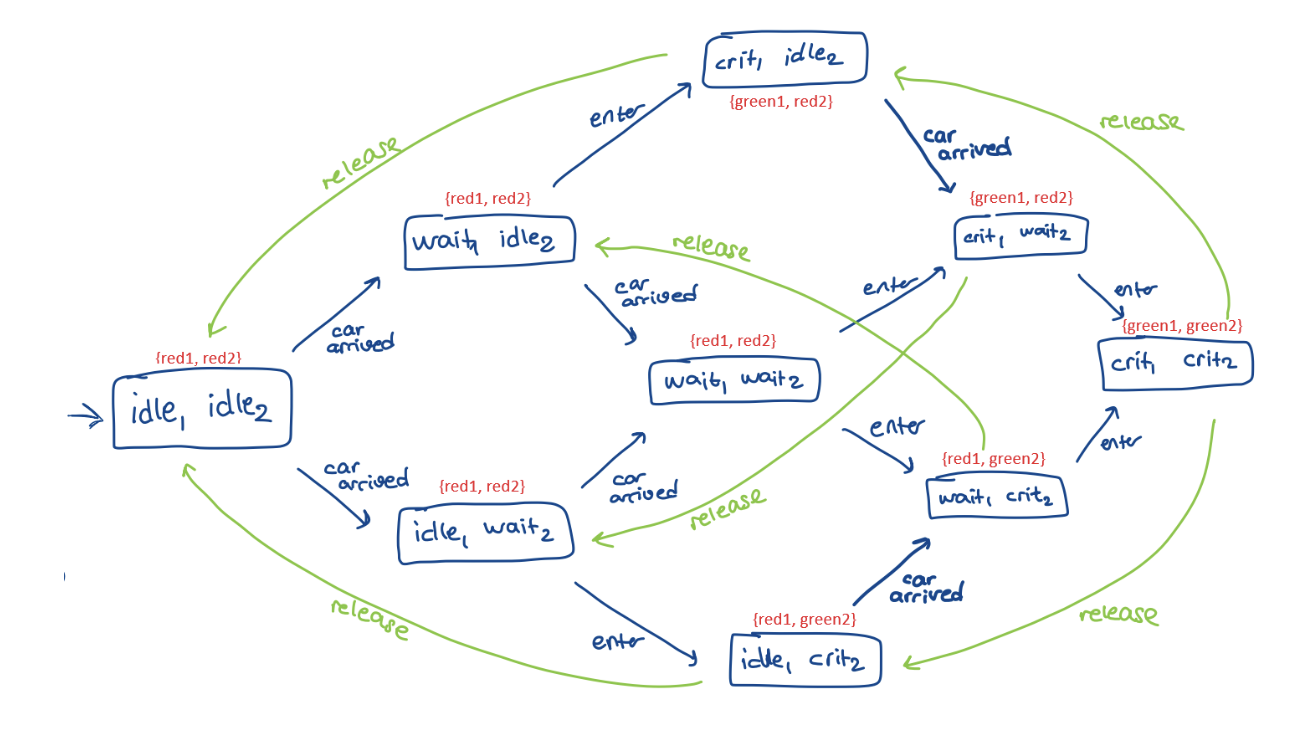
\includegraphics[width=5in]{images/3a.png}
        \caption{Interleaving transition systems $TS_1 | | | TS_2$}
        \label{fig:2a}
    \end{figure}

    \item{The traffic lights do not synchronize with each other, but they both synchronize
with the arbiter.}
    \begin{figure}[!htb]
        \centering
        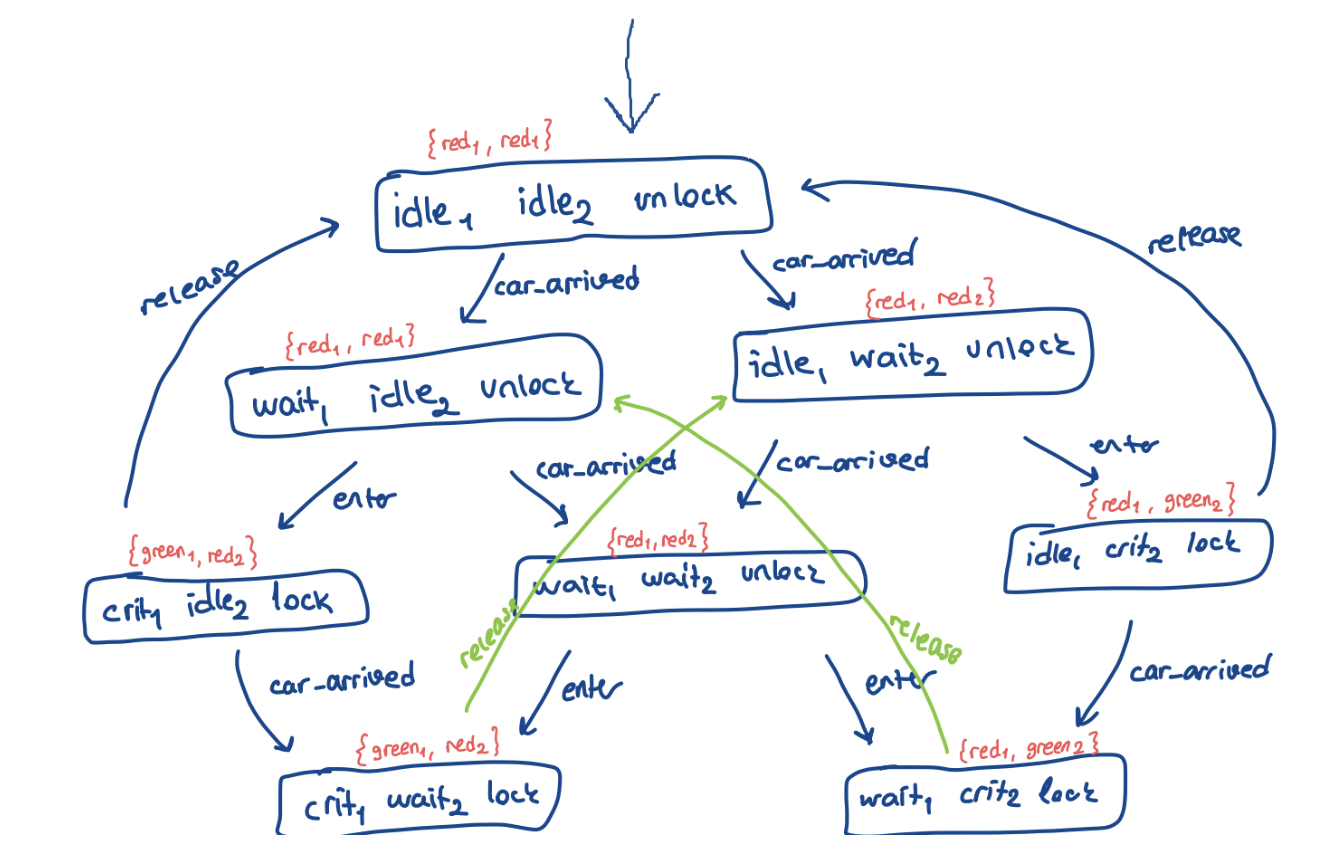
\includegraphics[width=5in]{images/3b.png}
        \caption{Parallel composition of systems $(TS_1 | | | TS_2)$ $| |$ Arbiter}
        \label{fig:2a}
    \end{figure}

    \item{Yes, the system is safe when synchronized with an Arbiter. There is no such a state where the atomic proposition is $\{\text{green}_1, \text{green}_2\}$.}\\
    However, in this design, the lights immediately switch from green to red. We would expect another state(s), e.g. a yellow light state, which would result in a slower and safer switch from green to red. 
\end{enumerate}


\end{document}